\documentclass{article}\usepackage[]{graphicx}\usepackage[]{color}
%% maxwidth is the original width if it is less than linewidth
%% otherwise use linewidth (to make sure the graphics do not exceed the margin)
\makeatletter
\def\maxwidth{ %
  \ifdim\Gin@nat@width>\linewidth
    \linewidth
  \else
    \Gin@nat@width
  \fi
}
\makeatother

\definecolor{fgcolor}{rgb}{0.345, 0.345, 0.345}
\newcommand{\hlnum}[1]{\textcolor[rgb]{0.686,0.059,0.569}{#1}}%
\newcommand{\hlstr}[1]{\textcolor[rgb]{0.192,0.494,0.8}{#1}}%
\newcommand{\hlcom}[1]{\textcolor[rgb]{0.678,0.584,0.686}{\textit{#1}}}%
\newcommand{\hlopt}[1]{\textcolor[rgb]{0,0,0}{#1}}%
\newcommand{\hlstd}[1]{\textcolor[rgb]{0.345,0.345,0.345}{#1}}%
\newcommand{\hlkwa}[1]{\textcolor[rgb]{0.161,0.373,0.58}{\textbf{#1}}}%
\newcommand{\hlkwb}[1]{\textcolor[rgb]{0.69,0.353,0.396}{#1}}%
\newcommand{\hlkwc}[1]{\textcolor[rgb]{0.333,0.667,0.333}{#1}}%
\newcommand{\hlkwd}[1]{\textcolor[rgb]{0.737,0.353,0.396}{\textbf{#1}}}%

\usepackage{framed}
\makeatletter
\newenvironment{kframe}{%
 \def\at@end@of@kframe{}%
 \ifinner\ifhmode%
  \def\at@end@of@kframe{\end{minipage}}%
  \begin{minipage}{\columnwidth}%
 \fi\fi%
 \def\FrameCommand##1{\hskip\@totalleftmargin \hskip-\fboxsep
 \colorbox{shadecolor}{##1}\hskip-\fboxsep
     % There is no \\@totalrightmargin, so:
     \hskip-\linewidth \hskip-\@totalleftmargin \hskip\columnwidth}%
 \MakeFramed {\advance\hsize-\width
   \@totalleftmargin\z@ \linewidth\hsize
   \@setminipage}}%
 {\par\unskip\endMakeFramed%
 \at@end@of@kframe}
\makeatother

\definecolor{shadecolor}{rgb}{.97, .97, .97}
\definecolor{messagecolor}{rgb}{0, 0, 0}
\definecolor{warningcolor}{rgb}{1, 0, 1}
\definecolor{errorcolor}{rgb}{1, 0, 0}
\newenvironment{knitrout}{}{} % an empty environment to be redefined in TeX

\usepackage{alltt}

\setlength{\parindent}{0pt} % Remove indent at new paragraphs
\setcounter{secnumdepth}{0}  % Remove section numbering at certain depth
\usepackage[round,sort]{natbib}
\usepackage{fixltx2e}
\usepackage{graphicx}  % For external pictures
\usepackage{float}
\usepackage{subfig}	% Add subfigures within figures
\usepackage{verbatim}
\usepackage[colorlinks=true,linkcolor=blue,citecolor=blue,urlcolor=blue]{hyperref}
\usepackage{amssymb,amsbsy,amsmath}
\usepackage{epsfig}
\usepackage[left=3cm,top=3cm,bottom=3.5cm,right=3cm]{geometry} % For easy document margins
\usepackage{fancyhdr} % For customization of header/footer
\usepackage{adjustbox}
\numberwithin{equation}{section} % Equation numbers relative to sections

\newcommand{\code}[1]{{\texttt{#1}}}
\newcommand{\pkg}[1]{{\texttt{#1}}}
\newcommand{\class}[1]{{\textit{#1}}}
\newcommand{\R}{{\normalfont\textsf{R }}{}}
\IfFileExists{upquote.sty}{\usepackage{upquote}}{}
\begin{document}

\title{Vignette: All About Tennis with tennisR}
\author{Justin Zwolski}
\date{\pkg{tennisR} version 1.0.0 , 2015-11-15 }
\maketitle

\tableofcontents
\setcounter{footnote}{1} \footnotetext{This \LaTeX\ vignette document is created using the \R function \code{Sweave} on the \R package \pkg{tennisR}. It is automatically downloaded with the package and can be accessed with the \R command \code{vignette("tennisR")}.}  \newpage
\setlength{\parskip}{10pt} % Inter-paragraph spacing



\section{Introduction}

\subsection{What is tennisR?} 

Analytics is becoming more and more popular in tennis.  Statistics from each match are being collected, and can be used to find ways to improve a player's performance.  The \pkg{tennisR} package provides an easy way to put match statistics into a database form that can be used for analysis.  This package also can compute player ratings for any given time period, and make predictions based on these ratings.  The available functions in the \pkg{tennisR} package and a detailed explanation of their usage will be discussed in this vignette.

\subsection{Data Collection}

The \pkg{tennisR} package provides an initial dataset of match statistics.  These statistics are collected from the ATP World Tour website, which is the website for the men's professional tennis association.  Information about each tournament can be found in the Results Archive page.  Within this page, the player draw for each tournament shows all the player matchups and displays the score for each match as a hyperlink.  When the hyperlink is clicked on, a pop-up window opens displaying information about each match, as well as all the statistics.

The base dataset in the \pkg{tennisR} package contains all matches for the 2013 and 2014 full seasons, as well as matches in 2015 up to and including the U.S. Open, for a total of 7,327 matches.  Every match is given two rows, one row of match statistics for each player.  There are a total of 46 variables in the dataset.

\begin{knitrout}
\definecolor{shadecolor}{rgb}{0.969, 0.969, 0.969}\color{fgcolor}\begin{kframe}


{\ttfamily\noindent\itshape\color{messagecolor}{\#\# Loading required package: XML\\\#\# Loading required package: RCurl\\\#\# Loading required package: bitops\\\#\# \\\#\# Attaching package: 'plyr'\\\#\# \\\#\# The following object is masked from 'package:lubridate':\\\#\# \\\#\#\ \ \ \  here}}\end{kframe}
\end{knitrout}

\begin{knitrout}
\definecolor{shadecolor}{rgb}{0.969, 0.969, 0.969}\color{fgcolor}\begin{kframe}
\begin{alltt}
\hlkwd{data}\hlstd{(MatchStats)}
\hlstd{MatchStats[}\hlkwd{c}\hlstd{(}\hlnum{1}\hlstd{,}\hlnum{2}\hlstd{),}\hlkwd{c}\hlstd{(}\hlnum{1}\hlopt{:}\hlnum{8}\hlstd{)]}
\end{alltt}
\begin{verbatim}
##      MatchID Year       Date              Tournament Surface       Round
## 1700       1 2013 2013-02-25 Abierto Mexicano Telcel    Hard Round of 32
## 2288       1 2013 2013-02-25 Abierto Mexicano Telcel    Hard Round of 32
##            Player     Opponent
## 1700 David Ferrer Antonio Veic
## 2288 Antonio Veic David Ferrer
\end{verbatim}
\begin{alltt}
\hlkwd{dim}\hlstd{(MatchStats)}
\end{alltt}
\begin{verbatim}
## [1] 14654    46
\end{verbatim}
\end{kframe}
\end{knitrout}


The first few variables provide information about the specific tournament and match.  The majority of the variables are the match statistics, which include serving, returning, and overall statistics.  An example of one of the serving statistics is first serve percentage, the percentage of first serves in play.

\begin{knitrout}
\definecolor{shadecolor}{rgb}{0.969, 0.969, 0.969}\color{fgcolor}\begin{kframe}
\begin{verbatim}
##            Player     Opponent First_Serve_Per First_Serve_Per_Diff
## 1700 David Ferrer Antonio Veic              60                   -2
## 2288 Antonio Veic David Ferrer              62                    2
\end{verbatim}
\end{kframe}
\end{knitrout}

Most of the statistics also have a calculated difference associated with them.  This is the difference in percentage of a statistic between two players in the same match.

Given the initial dataset of match statistics, graphs can be produced to look at trends among players, tournaments, or any variable in the dataset.  The following graph shows Andy Murray's first serve percentage from June 1, 2015 to the end of his U.S. Open run in early September.

\begin{knitrout}
\definecolor{shadecolor}{rgb}{0.969, 0.969, 0.969}\color{fgcolor}

{\centering 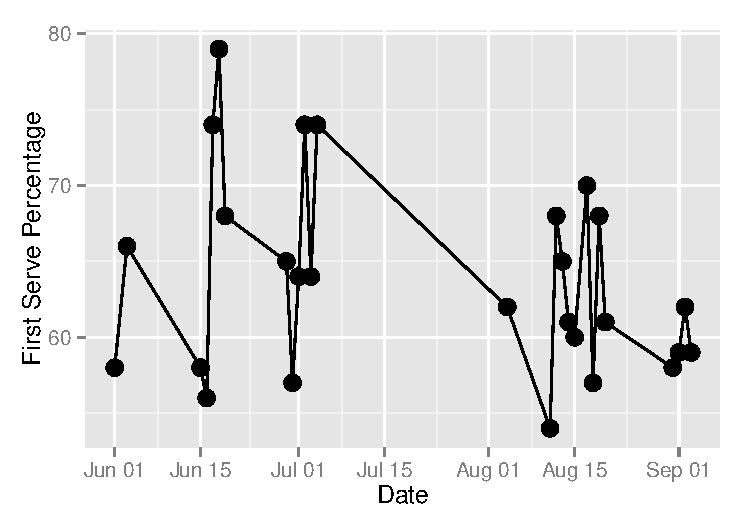
\includegraphics[width=\maxwidth]{figure/murray-1} 

}



\end{knitrout}

\section{Available Functions}

There are functions available in the \pkg{tennisR} package regarding match statistics, elo ratings, and predictions.  Each function is covered in detail, showing some examples, and the required format for the function inputs.

\subsection{NewMatchStats}

The \texttt{NewMatchStats} function allows the user to expand the original dataset in the package.  While the base dataset only contains matches from 2013 to the 2015 U.S. Open, matches from any tournament can be added to this dataset via the \texttt{NewMatchStats} function.  There is only one input to the \texttt{NewMatchStats} function.  This input is the website for a tournament.  The input can also include multiple websites.  In this case, the websites would need to be grouped together in a vector in order for the function to recognize each individual website.  As described above, the \pkg{tennisR} package uses data from the ATP World Tour website.  Therefore, the \texttt{NewMatchStats} function only has the ability to read tournament information from ATP websites.  

For example, to create a dataset of match statistics for the 2015 ATP World Tour Masters 1000 Series tournament in Shanghai, which occurred after the 2015 U.S. Open, the following input to the \texttt{NewMatchStats} function would be needed:

\begin{knitrout}
\definecolor{shadecolor}{rgb}{0.969, 0.969, 0.969}\color{fgcolor}\begin{kframe}
\begin{alltt}
\hlkwd{NewMatchStats}\hlstd{(}\hlstr{"http://www.atpworldtour.com/en/scores/archive/shanghai/5014/2015/draws"}\hlstd{)}
\end{alltt}
\end{kframe}
\end{knitrout}

Running this line of code would produce a dataframe of match statistics just for the tournament in Shanghai.  The dimensions of this dataframe are 110 by 46.  The number of variables is the same number as in the original dataset, which is to be expected.  Since two rows are used for each match, 55 matches were played during the tournament in Shanghai.

These match statistics can then easily be combined with the base dataset by using the rbind command.

\subsection{MatchResultselo}

The rest of the functions in the \pkg{tennisR} package relate to player ratings.  The ATP World Tour does have an official player ranking list, but this ranking is based on a yearly summation of points.  The chosen rating system for the \pkg{tennisR} package, the elo rating system, allows ratings to be calculated between any given time period.  In the elo rating system, each player is assigned an initial rating.  A player's rating changes each match, depending on the result.  The winning player will "take away" points from the losing player, thus increasing his player rating.  The losing player will lose points, thus decreasing his player rating.  The difference in elo rating between two players determines how many points are "transferred" from the losing player to the winning player.  However, if there is a large gap in points between players, and the higher rated player wins the match, very few points will be lost by the losing player since he was expected to lose the match.  If the lower rated player actually did win the match, many points would be transferred from the losing player to the winning player, thus increasing the player rating for the winner substantially.

The \pkg{PlayerRatings} package by Alec Stephenson has a built in function that calculates elo ratings.  Since the elo rating system is only based on the result of each match, the full dataset of match statistics must be modified.  The \texttt{MatchResultselo} function in the \pkg{tennisR} package takes a full dataset of match statistics, and keeps only the four variables that are needed to calculate the elo ratings.  The first variable is the number of days from a specific date.  This starting date in the \texttt{MatchResultselo} function is December 30, 2012, since this is the day of the first match in the base dataset.  The next two variables are the names of the two players, one listed as the "Player", and the other listed as the "Opponent".  The final variable is the result of the match.  The result of the match is a numeric variable, where a "1" represents the "Player" winning the match, and a "0" represents the "Opponent" winning the match.  Since the result of the match can be specified in one row, there is only one row per match in this new dataset.  Example output from the \texttt{MatchResultselo} function is shown below:

\begin{knitrout}
\definecolor{shadecolor}{rgb}{0.969, 0.969, 0.969}\color{fgcolor}\begin{kframe}
\begin{alltt}
\hlstd{matchresults} \hlkwb{<-} \hlkwd{MatchResultselo}\hlstd{(MatchStats[MatchStats}\hlopt{$}\hlstd{Year}\hlopt{==}\hlnum{2014}\hlstd{,])}
\hlkwd{head}\hlstd{(matchresults)}
\end{alltt}
\begin{verbatim}
##       Day          Player               Opponent Result
## 11217 421    David Ferrer      Mikhail Kukushkin      1
## 11316 421 Feliciano Lopez Edouard Roger-Vasselin      1
## 13216 421     Sam Querrey             Tigre Hank      1
## 17216 421  Kevin Anderson        Stephane Robert      1
## 19215 421    Ivo Karlovic             John Isner      1
## 25213 421       Dudi Sela        Alejandro Falla      1
\end{verbatim}
\end{kframe}
\end{knitrout}

The first column, Day, is the number of days from December 30, 2012.  Since the result is a "1" for each of the six matches, the player listed first in each row is the winner of the match.

\subsection{Eloratings\_nostatus}

Once the \texttt{MatchResultselo} function is applied to a dataset of match statistics, elo ratings can be calculated for any given time frame.  The first function that calculates elo ratings, the \texttt{Eloratings\_nostatus} function, requires three inputs.  The first two inputs are the beginning and end dates for the range in which the elo ratings will be calculated.  These two dates must be in a specific format, such as 2015-07-15, which would represent July 7, 2015.  The third input is a dataframe of match results after the \texttt{MatchResultselo} function has been run.  The \texttt{Eloratings\_nostatus} function initially finds the number of days between the inputted beginning date and December 30, 2012, as well as the number of days between the inputted end date and December 30, 2012.  Once the number of days is found, the third input representing the dataframe of match results is subsetted to only include matches between these two number of days.  The elo ratings for players that have played matches between these days is then calculated, given an initial rating of zero for each player.  No status occurs in the function name, since the elo ratings are calculated only between the specified beginning and end date.  The \texttt{Eloratings\_nostatus} function returns a list of elo ratings, and a list of matches played between the beginning and end dates.  In the list of elo ratings, the first row corresponds to the highest rated player, and the last row corresponds to the lowest rated player.  An example of this function is shown below:



\begin{knitrout}
\definecolor{shadecolor}{rgb}{0.969, 0.969, 0.969}\color{fgcolor}\begin{kframe}
\begin{alltt}
\hlstd{elo} \hlkwb{<-} \hlkwd{Eloratings_nostatus}\hlstd{(}\hlstr{"2014-03-01"}\hlstd{,}\hlstr{"2014-04-01"}\hlstd{,matchresults)}
\hlkwd{head.list}\hlstd{(elo[[}\hlnum{1}\hlstd{]][}\hlnum{1}\hlstd{] ,}\hlkwc{n}\hlstd{=}\hlnum{10}\hlstd{)}
\end{alltt}
\begin{verbatim}
## $ratings
##                   Player   Rating Games Win Draw Loss Lag
## 1         Novak Djokovic 97.81916    12  10    0    2   0
## 2          Roger Federer 75.66310    10   8    0    2   2
## 3          Kei Nishikori 73.05335     7   6    0    1   1
## 4    Alexandr Dolgopolov 63.64769     9   7    0    2   2
## 5          Tomas Berdych 61.09983     6   5    0    1   1
## 6           Milos Raonic 51.97383     8   6    0    2   2
## 7             John Isner 50.97044     8   6    0    2   3
## 8       Julien Benneteau 49.67705     8   6    0    2   4
## 9            Andy Murray 42.31281     7   5    0    2   2
## 10 Roberto Bautista Agut 36.14540     7   5    0    2   4
\end{verbatim}
\end{kframe}
\end{knitrout}

\subsection{Eloratings\_status}

The second function that calculates elo ratings, the \texttt{Eloratings\_status} function, also requires three inputs.  The first two inputs are the beginning and end dates for the range in which the elo ratings will be calculated.  These two dates must be in a specific format, such as 2015-07-15, which would represent July 15, 2015.  The third input is a dataframe of match results after the \texttt{MatchResultselo} function has been run.  Instead of calculating elo ratings for matches only within the specified dates, the \texttt{Eloratings\_status} function also uses completed matches up to one month prior to the beginning date specified in the input.  Elo ratings are calculated first for these "prior" matches, and these ratings serve as the "status" for the elo ratings between the two specified dates.  This means that the elo ratings for these prior matches now serve as the initial rating when calculating the elo ratings between the two specified dates.  Any player for which elo ratings were calculated for the "prior" matches, would also show up in the overall elo ratings between the two specified dates, regardless if the player actually did play a match between those dates.  Any players who didn't play in any of the prior matches would receive an initial rating of zero, similar to the previous function.  Updating the "status" of the elo ratings up to one month back can account for injuries to players, or players who missed matches due to other reasons.  The \texttt{Eloratings\_status} function returns a list of elo ratings, and a list of matches played between the beginning and end dates, plus up to one month prior to the beginning date.  The following code shows an example for the \texttt{Eloratings\_status} function using the same inputs as the example for the previous function.

\begin{knitrout}
\definecolor{shadecolor}{rgb}{0.969, 0.969, 0.969}\color{fgcolor}\begin{kframe}
\begin{alltt}
\hlstd{elo} \hlkwb{<-} \hlkwd{Eloratings_status}\hlstd{(}\hlstr{"2014-03-01"}\hlstd{,}\hlstr{"2014-04-01"}\hlstd{,matchresults)}
\hlkwd{head.list}\hlstd{(elo[[}\hlnum{1}\hlstd{]][}\hlnum{1}\hlstd{] ,}\hlkwc{n}\hlstd{=}\hlnum{10}\hlstd{)}
\end{alltt}
\begin{verbatim}
## $ratings
##                 Player    Rating Games Win Draw Loss Lag
## 1        Tomas Berdych 141.73391     6   5    0    1   1
## 2        Roger Federer 128.69225    10   8    0    2   2
## 3          Marin Cilic 127.58707     4   2    0    2   5
## 4         David Ferrer 121.06077     3   2    0    1   3
## 5        Kei Nishikori 120.40146     7   6    0    1   1
## 6  Alexandr Dolgopolov 113.05707     9   7    0    2   2
## 7       Novak Djokovic 106.64354    12  10    0    2   0
## 8        Fabio Fognini  95.02590     6   4    0    2   3
## 9       Ernests Gulbis  87.68573     5   3    0    2   5
## 10        Rafael Nadal  77.86456     8   5    0    3   0
\end{verbatim}
\end{kframe}
\end{knitrout}

This top ten list of players based on elo ratings shows that Tomas Berdych is the top rated player, instead of Novak Djokovic.  The number of wins, losses, and total games are the same for both sets of ratings, because these are the matches played between March 1, 2014 and April 1, 2014.  The difference in the ratings is due to the fact that the \texttt{Eloratings\_status} function uses prior match results from February 1, 2014 to February 28, 2014 to set the initial ratings.

\subsection{Eloratingstodf}

The \texttt{Eloratingstodf} function is a very simple function, but is useful in analyzing elo ratings.  

critical in making predictions based on calculated elo ratings.  Since the elo ratings are returned in list form, which can be difficult to work with, the \texttt{Eloratingstodf} function converts the elo ratings into a dataframe.   the prediction functions require the elo ratings to be 

\subsection{Predict\_nostatus}

a

\subsection{Predict\_status}

a

\section{Case Studies}

\subsection{2015 Miami Open}



\section{Conclusion}

\section{Future Work}

Work on predicting a full tournament, where the website for the tournament is used in a function, and it returns probabilities for all the matchups.

Work on Shiny app, and make it part of the \pkg{tennisR} package

\section{Bibliography}

\end{document}
